\begin{circuitikz}{scale=1}
\node[anchor=south east] at (0,0) {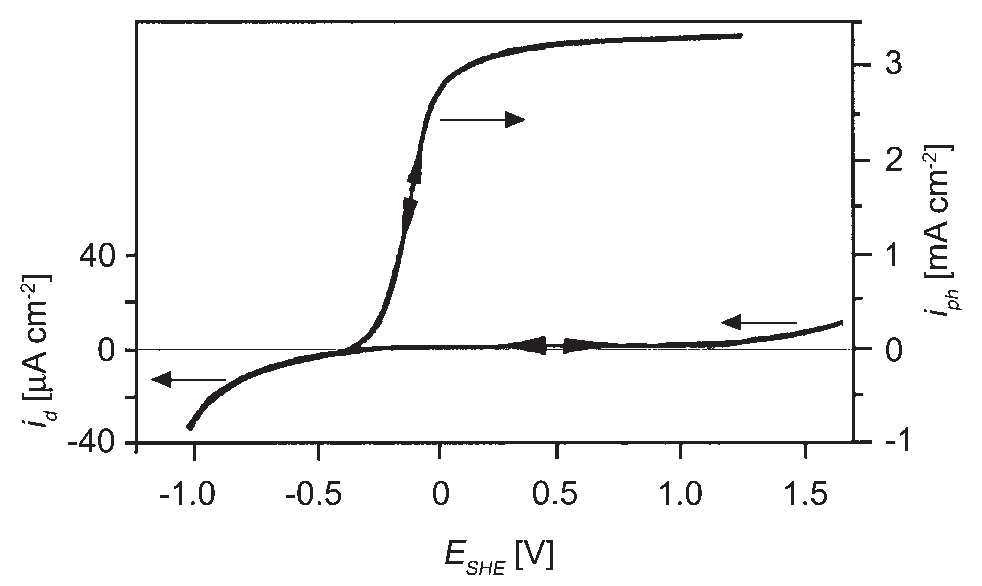
\includegraphics{figures/Plieth_2008-Fig9_10a.png}};
\node[anchor=center] at (-3,0) {a)};
\node[anchor=south west] at (0,0) {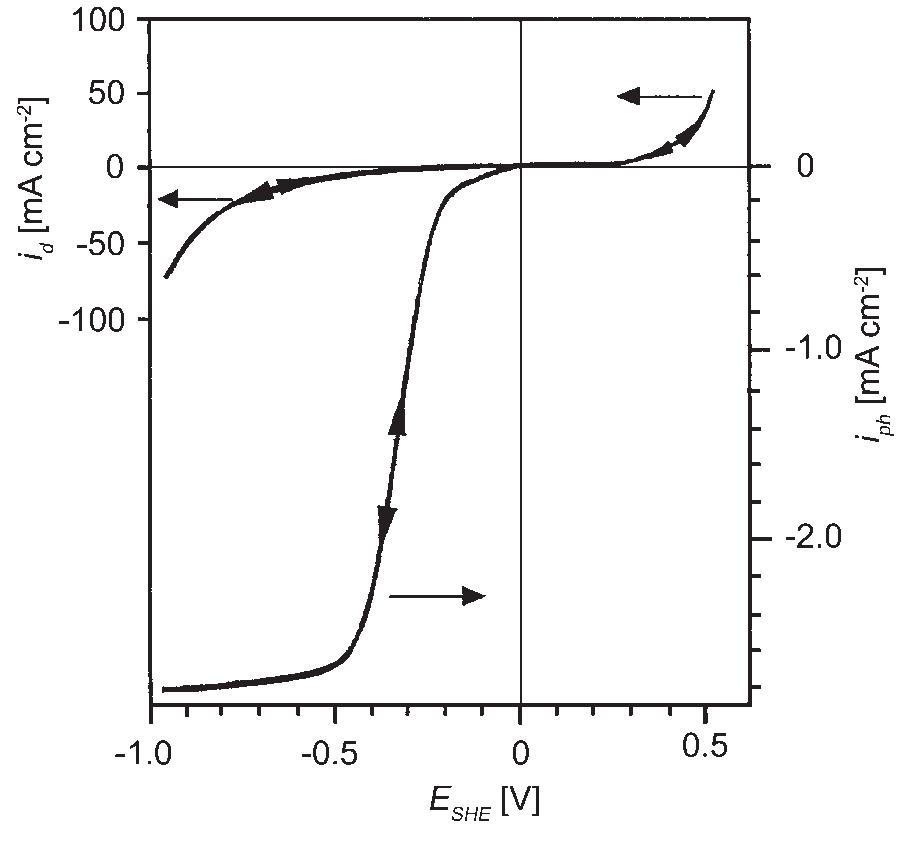
\includegraphics{figures/Plieth_2008-Fig9_10b.png}};
\node[anchor=center] at (3,0) {b)};

\draw[-Stealth, blue, ultra thick] (-4.6,4.1) -- ++(1.5,0.0) node[at end, right, fill=white] {Anodic $i_{ph}$};
\draw[-Stealth, red, ultra thick] (3.5,2.25) -- ++(1.5,0) node[at end, right, fill=white] {Cathodic $i_{ph}$};

\end{circuitikz}